
%%% Local Variables: 
%%% mode: latex
%%% TeX-master: t
%%% End: 

\documentclass[dvipsnames, svgnames, mode=present, paper=screen, size=9pt,
style=husky]{powerdot}
\usepackage{calc}
\usepackage{amsmath}
\usepackage{fancybox}
\usepackage{fancyvrb}
\setlength{\shadowsize}{1pt}
\usepackage{mflogo}
\usepackage{shapepar}
%\usepackage{fourier}
\usepackage{CJK,CJKpunct}

\usepackage{tikz}
%\usepackage{pgflibraryarrows}
%\usepackage{pgflibrarysnakes}
\usepackage{pstricks}
\usepackage{pst-node}

\hypersetup{CJKbookmarks=true}
\makeatletter
 \def\beamer@activecjk{
    % Activate all >128 characters. 
    \count@=127
    \@whilenum\count@<255 \do{%
      \advance\count@ by 1
      \lccode`\~=\count@
      \catcode\count@=\active
      \lowercase{\def~{\kern1ex}}
    }
  } 
\beamer@activecjk
\makeatother

\pdsetup{%
theslide=\arabic{slide}~/~\pageref*{lastslide},
lf=\href{http://thuthesis.sf.net}{ThuThesis},
rf=\href{mailto:xueruini@gmail.com}{Xue Ruini},
randomdots,
dbright=70,
dmindots=6,dmaxdots=9,
dminsize=5pt,dmaxsize=20pt,
logopos={.04\slidewidth,.19\slideheight}}

\graphicspath{{figures/}}


\newcommand{\song}{\CJKfamily{song}}    % 宋体
\newcommand{\fs}{\CJKfamily{fs}}        % 仿宋体
\newcommand{\kai}{\CJKfamily{kai}}      % 楷体
\newcommand{\hei}{\CJKfamily{hei}}      % 黑体
\newcommand{\li}{\CJKfamily{li}}        % 隶书
\newcommand{\you}{\CJKfamily{you}}      % 幼圆


\makeatletter
\newlength\thu@linespace
\newcommand{\thu@choosefont}[2]{%
      \setlength{\thu@linespace}{#2*\real{#1}}%
      \fontsize{#2}{\thu@linespace}\selectfont}
\newcommand{\chuhao}[1][\baselinestretch]{\thu@choosefont{#1}{42bp}}
\newcommand{\xiaochu}[1][\baselinestretch]{\thu@choosefont{#1}{36bp}}
\newcommand{\yihao}[1][\baselinestretch]{\thu@choosefont{#1}{26bp}}
\newcommand{\xiaoyi}[1][\baselinestretch]{\thu@choosefont{#1}{24bp}}
\newcommand{\erhao}[1][\baselinestretch]{\thu@choosefont{#1}{22bp}}
\newcommand{\xiaoer}[1][\baselinestretch]{\thu@choosefont{#1}{18bp}}
\newcommand{\sanhao}[1][\baselinestretch]{\thu@choosefont{#1}{16bp}}
\newcommand{\xiaosan}[1][\baselinestretch]{\thu@choosefont{#1}{15bp}}
\newcommand{\sihao}[1][\baselinestretch]{\thu@choosefont{#1}{14bp}}
\newcommand{\banxiaosi}[1][\baselinestretch]{\thu@choosefont{#1}{13bp}}
\newcommand{\xiaosi}[1][\baselinestretch]{\thu@choosefont{#1}{12bp}}
\newcommand{\dawu}[1][\baselinestretch]{\thu@choosefont{#1}{11bp}}
\newcommand{\wuhao}[1][\baselinestretch]{\thu@choosefont{#1}{10.5bp}}
\newcommand{\xiaowu}[1][\baselinestretch]{\thu@choosefont{#1}{9bp}}
\newcommand{\liuhao}[1][\baselinestretch]{\thu@choosefont{#1}{7.5bp}}
\newcommand{\xiaoliu}[1][\baselinestretch]{\thu@choosefont{#1}{6.5bp}}
\newcommand{\qihao}[1][\baselinestretch]{\thu@choosefont{#1}{5.5bp}}
\newcommand{\bahao}[1][\baselinestretch]{\thu@choosefont{#1}{5bp}}
\makeatother

\makeatletter
\def\psRotation#1(#2,#3)#4{%
  \rput{#1}(#2,#3){%
    \psellipticarc[linewidth=.4pt]{->}(0,-0.1)(0.6,0.15){120}{70}
    \ifdim#1pt>\z@\rput[l]{*0}(0.675,0){#4}\else\rput[l](0.675,0){#4}\fi
  }%
}

\newcommand{\ziju}[1][2pt]{\renewcommand{\CJKglue}{\hskip #1}}
\def\thuthesis{\textsc{Thu}\textsc{Thesis}}
\def\cmd#1{\texttt{\color{DarkBlue}\footnotesize $\backslash$#1}}
\def\env#1{\texttt{\color{DarkBlue}\footnotesize #1}}
\def\cmdxmp#1#2#3{\small{\texttt{\color{DarkBlue}$\backslash$#1}\{#2\}\hspace{1em}\\ $\Rightarrow$\hspace{1em} {#3}\par\vskip1em}}
\newcommand\mysb[2][Indigo]{\Pisymbol{ding}{19}\hskip5pt\shadowbox{\color{#1}\li #2}}

\newcommand{\wt}{\widetilde}
\newcommand{\wh}{\widehat} 
\newcommand{\envert}[1]{\left\lvert#1\right\rvert}
\let\abs=\envert 

% \RecustomVerbatimEnvironment{Verbatim}{Verbatim}%
%   {frame=single, baselinestretch=1,fontsize=\footnotesize}

% \DefineVerbatimEnvironment{MyVerbatim}{Verbatim}%
%  {formatcom=\color{DarkViolet},rulecolor=\color{Gray},%
%   frame=single, baselinestretch=1,fontsize=\footnotesize}

\DefineVerbatimEnvironment{MyVerbatim}{Verbatim}%
  {frame=single, framerule=0.3mm, rulecolor=\color{red!75!green!50!blue}, 
   fillcolor=\color{red!75!green!50!blue!15},framesep=.5mm,baselinestretch=1,
   fontsize=\footnotesize}
\DefineVerbatimEnvironment{YourVerbatim}{Verbatim}%
  {frame=single, framerule=0.3mm, rulecolor=\color{red!85!green!60},baselinestretch=1,
   fillcolor=\color{red!85!green!10},framesep=.5mm,fontsize=\footnotesize}

\long\def\mypauseverb<#1>#2{\onslide{#1}{{\renewcommand{\baselinestretch}{1.1}\color{DarkViolet}\footnotesize
      #2}}}
\long\def\mypauseverbatim<#1>#2{%
  \begin{SaveVerbatim}{mypause}#2\end{SaveVerbatim}%
  \mypauseverb<#1>{\Useverbatim{#2}}}
\long\def\myitem<#1>#2{\onslide{#1}{\tikz\shade[ball color=orange] (0em, 0.5em) circle (0.5em); \hspace{2pt} #2\par}}

\renewcommand{\baselinestretch}{1.3}

\begin{document}
\begin{CJK*}{GBK}{song}
\def\version{v3.0}
\title{\hei\Huge ThuThesis~使用向导~\version}
\author{\fs 薛瑞尼\\[5pt]\texttt{LittleLeo@newsmth}\\[10pt]\li 清华大学~~计算机系~~高性能所}
\date{\the\year.\the\month.\the\day}
\maketitle

\pdsetup{logocmd={\includegraphics[scale=0.05]{thu-fig-logo.pdf}}}

\begin{slide}[toc=, bm=]{目录}
\tableofcontents[type=1, content=sections]
\end{slide}


\section{介绍}
\begin{slide}[]{\TeX{} 是什么?}
$\mbox{\TeX} = \tau\epsilon\chi$['tek]
  \begin{itemize}
  \item 上世纪~70 年代,Stanford 大学~Donald E. Knuth 教授发明
  \item 西方电子排版界的革命
  \item 漂亮、美观、大方、稳定、通用
  \item 特长:公式~~ (其它方面同样出色)
  \end{itemize}
\medskip

\centering
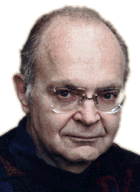
\includegraphics[scale=0.3]{knuth.png}\hspace{2cm}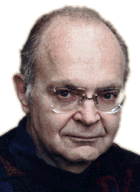
\includegraphics[scale=0.11]{knuth.png}%texbook.eps

\begin{equation}
\det\mathbf{K}(t=1,t_1,\dots,t_n)=\sum_{I\in\mathbf{n}}(-1)^{\envert{I}}
\prod_{i\in I}t_i\prod_{j\in I}(D_j+\lambda_jt_j)\det\mathbf{A}
^{(\lambda)}(\overline{I}|\overline{I})=0.
\end{equation} 
\end{slide}

\begin{slide}{\LaTeX{} 是什么?}
\LaTeX $=$ Lamport \TeX~['latek] (or ['leitek])\footnote{\url{http://lists.fas.harvard.edu/pipermail/gov1760-l/2002-October/000465.html}}
  \begin{itemize}
  \item \TeX{} 包括~900 多条命令,使用不便
  \item Leslie Lamport 开发~\LaTeX{} 降低使用门槛
  \item 本质上仍然是~\TeX{}
  \item 最广泛的~\TeX{} 宏包,几乎所有国际期刊会议
  \item 许多著名大学都有~\LaTeX{} 论文模板
  \end{itemize}
\bigskip

\centering
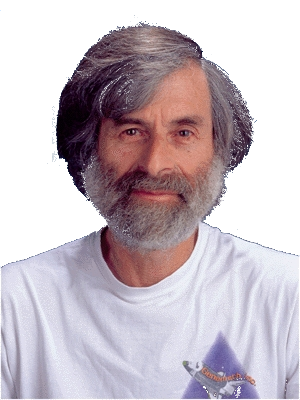
\includegraphics[scale=0.2]{lamport.png}\hspace{2cm}\scalebox{2}{\LaTeX}
\end{slide}

\begin{slide}{\thuthesis{} 是什么?}
  \onslide*{1}{\vspace*{-0.3cm}\heartpar{\textbf{\thuthesis} is a \LaTeX{}
      package aiming to facilitate the thesis writing for bachelors, masters and
      doctors of Tsinghua University.  By now, \thuthesis\  has been widely used
      among lots of \TeX\ zealots who do not want to format their several years'
      hard work with the infamous  MS WORD. I created \thuthesis\ in the summer
      of 2005, and made it more useful and stable in the spring of 2006. To be
      frank, \thuthesis\ is not going to fight with MS WORD, because in my
      opinion, ``The best tool depends on you''. It is hard to persuade all
      students to give up MS WORD and turn to \TeX, but I'd like to encourage
      them through my efforts. Actually, \thuthesis\ is in its initial step now,
      as an infant, \thuthesis\ needs your help very much, and it is very kind
      of you to contribute and promote it. \textbf{Xue Ruini}}}

\onslide*{2}{\thuthesis —— 清华大学学位论文~\LaTeX{} 模板
  \begin{itemize}
  \item 最早:王磊~(2004.4)
  \item 2005~硕士毕业,始有~$\Rightarrow$ \blue{报盘版}
  \item 不断修改更新:$\Rightarrow$ \thuthesis-2.0 (2005/12/20)
  \item 首次融合本科、硕士、博士论文格式:$\Rightarrow$ \thuthesis-2.1 (2006/3/4)
  \item 如今:\thuthesis-3.0 (2007/05/13)
  \end{itemize}
\medskip

\centering
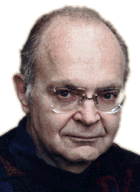
\includegraphics[width=3cm]{knuth.png}\hspace{1cm}%master.eps
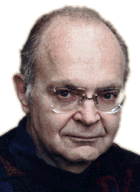
\includegraphics[width=2.6cm]{knuth.png}\\%contents.eps
{\footnotesize 封面}\hspace{3.3cm} {\footnotesize 目录}}
\end{slide}

\begin{slide}{为什么不是~WORD?}
  \begin{itemize}
  \item MS WORD 是世界上最流行的“字处理软件”,但不是专业的出版软件
  \item 二进制封闭格式
  \item 所见即所得~(WYSIWYG)
  \item 简单直观、容易上手,适合日常使用、简单文档
  \item 但进阶慢,掌握高级功能不易
  \item 处理长文档需要丰富的经验,否则将是一场恶梦
  \item 最关键的:移植性不好、稳定性受怀疑、崩溃是常事
  \item 其它:你需要付钱~(如果我们不想吃~Bill Gates 的官司)
  \end{itemize}
  \bigskip
\centering
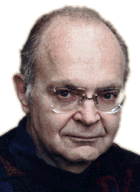
\includegraphics[width=3cm]{knuth.png}% think.eps
\end{slide}

\begin{slide}{为什么是~\TeX ?}
  \begin{itemize}
  \item 专业的排版系统\\
\twocolumn[lcolwidth=0.3\linewidth, rcolwidth=0.6\linewidth, topsep=0.5cm,bottomsep=0.5cm]{
    \begin{itemize}
    \item AMS
    \item IEEE
    \item SIAM
    \item Elsevier
    \end{itemize}}{
    \begin{itemize}
    \item Springer
  \item Kluwer Academic Publishers
    \item Cambridge University Press
    \item Reviews of Modern Physics
    \end{itemize}}

  \item 纯文本格式 
  \item 所想即所得~(WYTIWYG)
  \item 上手容易:\\
        花一个上午读~lshort,掌握基本~\LaTeX{} 就算掌握了~90%
  \item 进阶虽难,但一般用不着~(究竟什么是模板?见后文)
  \item 移植性好,稳定,如果崩溃,基本上是用户所致
  \item 如果真的发现问题,可以给~Knuth 发信,并得到~{\color{blue}$2^{n}$} 美分的奖励
  \end{itemize}
\end{slide}

\begin{slide}{\TeX{} Showcase (1)}
  \begin{itemize}
  \item 优美的公式
  \end{itemize}
  \begin{equation}
\begin{split}
f_{h,\varepsilon}(x,y)
&=\varepsilon\mathbf{E}_{x,y}\int_0^{t_\varepsilon}
L_{x,y_\varepsilon(\varepsilon u)}\varphi(x)\,du\\
&= h\int L_{x,z}\varphi(x)\rho_x(dz)\\
&\quad+h\biggl[\frac{1}{t_\varepsilon}\biggl(\mathbf{E}_{y}
  \int_0^{t_\varepsilon}L_{x,y^x(s)}\varphi(x)\,ds
  -t_\varepsilon\int L_{x,z}\varphi(x)\rho_x(dz)\biggr)\\
&\phantom{{=}+h\biggl[}+\frac{1}{t_\varepsilon}
  \biggl(\mathbf{E}_{y}\int_0^{t_\varepsilon}L_{x,y^x(s)}
    \varphi(x)\,ds -\mathbf{E}_{x,y}\int_0^{t_\varepsilon}
   L_{x,y_\varepsilon(\varepsilon s)}
   \varphi(x)\,ds\biggr)\biggr]\\
&=h\wh{L}_x\varphi(x)+h\theta_\varepsilon(x,y),
\end{split}
\end{equation} 

\begin{equation}
\begin{split}
 \abs{I_2}&=\left\lvert \int_{0}^T \psi(t)\left\{u(a,t)-\int_{\gamma(t)}^a
  \frac{d\theta}{k(\theta,t)}
  \int_{a}^\theta c(\xi)u_t(\xi,t)\,d\xi\right\}dt\right\rvert\\
&\le C_6\left\lvert \left\lvert f\int_\Omega\left\lvert \wt{S}^{-1,0}_{a,-}
  W_2(\Omega,\Gamma_l)\right\rvert\right\rvert
  \left\lvert \abs{u}\overset{\circ}\to W_2^{\wt{A}}
  (\Omega;\Gamma_r,T)\right\rvert\right\rvert.
\end{split}
\end{equation}
\end{slide}

\begin{slide}{\TeX{} Showcase (2)}
  \begin{itemize}
  \item 优美的公式
  \end{itemize}
{\delimiterfactor750
\begin{align}
\begin{split}\abs{I_1}
  &=\left\lvert \int_\Omega gRu\,d\Omega\right\rvert\\
&\le C_3\left[\int_\Omega\left(\int_{a}^x
  g(\xi,t)\,d\xi\right)^2d\Omega\right]^{1/2}\\
&\quad\times \left[\int_\Omega\left\{u^2_x+\frac{1}{k}
  \left(\int_{a}^x cu_t\,d\xi\right)^2\right\}
  c\Omega\right]^{1/2}\\
&\le C_4\left\lvert \left\lvert f\left\lvert \wt{S}^{-1,0}_{a,-}
  W_2(\Omega,\Gamma_l)\right\rvert\right\rvert
  \left\lvert \abs{u}\overset{\circ}\to W_2^{\wt{A}}
  (\Omega;\Gamma_r,T)\right\rvert\right\rvert.
\end{split}\label{eq:A}\\[10pt]
\begin{split}\abs{I_2}&=\left\lvert \int_{0}^T \psi(t)\left\{u(a,t)
  -\int_{\gamma(t)}^a\frac{d\theta}{k(\theta,t)}
  \int_{a}^\theta c(\xi)u_t(\xi,t)\,d\xi\right\}dt\right\rvert\\
&\le C_6\left\lvert \left\lvert f\int_\Omega
 \left\lvert \wt{S}^{-1,0}_{a,-}
  W_2(\Omega,\Gamma_l)\right\rvert\right\rvert
  \left\lvert \abs{u}\overset{\circ}\to W_2^{\wt{A}}
  (\Omega;\Gamma_r,T)\right\rvert\right\rvert.
\end{split}
\end{align}}  
\end{slide}

\begin{slide}{\TeX{} Showcase (3)}
  \begin{itemize}
  \item 精确的图形
  \end{itemize}
  \begin{minipage}{0.3\linewidth}    
\psset{unit=0.8cm}
  \begin{pspicture}(-1.75,-3)(3.25,4)
\psline[linewidth=0.25pt](0,0)(0,4)
\rput[tl]{0}(0.2,2){$\vec e_z$}
\rput[tr]{0}(-0.9,1.4){$\vec e$}
\rput[tl]{0}(2.8,-1.1){$\vec C_{ptm{ext}}$}
\rput[br]{0}(-0.3,2.1){$\theta$}
\rput{25}(0,0){%
  \psframe[fillstyle=solid,fillcolor=lightgray,linewidth=.8pt](-0.1,-3.2)(0.1,0)}
\rput{25}(0,0){%
  \psellipse[fillstyle=solid,fillcolor=yellow,linewidth=3pt](0,0)(1.5,0.5)}
\rput{25}(0,0){%
  \psframe[fillstyle=solid,fillcolor=lightgray,linewidth=.8pt](-0.1,0)(0.1,3.2)}
\rput{25}(0,0){\psline[linecolor=red,linewidth=1.5pt]{->}(0,0)(0.,2)}
\psRotation{0}(0,3.5){$\dot\phi$}
\psRotation{25}(-1.2,2.6){$\dot\psi$}
\psline[linecolor=red,linewidth=1.25pt]{->}(0,0)(0,2)
\psline[linecolor=red,linewidth=1.25pt]{->}(0,0)(3,-1)
\psline[linecolor=red,linewidth=1.25pt]{->}(0,0)(2.85,-0.95)
\psarc{->}{2.1}{90}{112.5}
\rput[bl](.1,.01){C}
\end{pspicture}
  \end{minipage}\hspace{1cm}
\begin{minipage}[t]{0.5\linewidth}  
\psset{unit=0.3cm}
\begin{pspicture}(1,2)(18,14)
%\psgrid[gridcolor=lightgray,subgriddiv=0,subgridcolor=lightgray]
%
\psline[linewidth=1pt,linecolor=black](6,0.5)(6,14)
\psline[linewidth=1pt,linecolor=black](1,8.5)(6,7)
\psline[linewidth=1pt,linecolor=black](1.5,5.5)(11,8.5)
%
\rput(17,3){$x$}
\rput(5.5,13){$y$}
\rput(10.5,8.75){$z$}
\rput(11,7.1){$\vec{r}$}
%
\psline[linewidth=1.5pt,linecolor=black]{<->}(6,7)(6,11.25)
\rput(5.35,9.4){$R$}
\psline[linewidth=1.5pt,linecolor=Green]{->}(6.5,12)(4.75,12)
\rput(7.5,12.8){ $I d\vec{l}$}
%
\psellipse[doubleline=true,doublecolor=yellow,doublesep=3pt,linecolor=blue](6,7)(3,4.5)
\psline[linewidth=1pt,linecolor=black](6,7)(17.5,3.5)
\psline[linewidth=1.5pt,linecolor=black]{->}(6,11.38)(11.95,5.225)
%
\psarc[linewidth=1.5pt,linecolor=gray](6,8){3.4}{85}{95}
%
\psline[linewidth=1.5pt,linecolor=gray]{->}(12,5.15)(12,8.15)
\psline[linewidth=1.5pt,linecolor=black]{->}(12,5.15)(15,7.25)
\psline[linewidth=1.5pt,linecolor=gray]{->}(12,5.15)(15,4.25)
%
\psline[linewidth=1pt,linecolor=black](12,8.15)(15,7.25)(15,4.25)
%
\Cnode*[linecolor=black,radius=0.1cm](12,5.15){a}
\rput(11.5,4.5){ $P$}
%
\rput(12.5,8.9){$dB_y$}
\rput(14.5,3.4){$dB_x$}
\rput(15.5,8){ $d \boldmath{\vec{B}}$}
%
\psarc[linewidth=1pt]{<->}(12,5){5.5}{133}{161}
\rput(7.2,8.5){ $\theta$}
\end{pspicture}
\medskip

\hspace{2cm}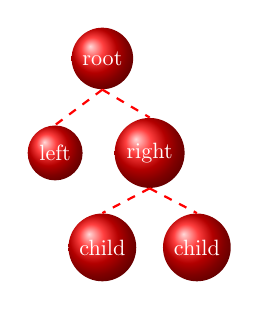
\begin{tikzpicture}
[parent anchor=south,child anchor=north,grow=south, scale=0.8]
\tikzstyle{every node}=[ball color=red,circle,text=white, scale=0.8]
\tikzstyle{edge from parent}=[draw,dashed,thick,red]
\node {root}
child {node {left}}
child {node {right}
child {node {child}}
child {node {child}}
};
\end{tikzpicture}
\end{minipage}
\end{slide}
\begin{note}{personal note}
text format
\end{note}

\section{模板是什么}

\begin{slide}{什么是模板?}
  \begin{itemize}
  \item 通俗地讲:已经建立好的框架
  \item 好的模板:使用户专注于内容
  \item 不应将大量时间消耗在调整框架上
  \end{itemize}
  \end{slide}

\begin{slide}{Office 的误导}  
\begin{itemize}
\item 很少有人会有意识地在~WORD 中使用模板
\item 定义自己的标题?定义自己的列表?定义自己的段落样式?
\item 自动化,还是手工调?
\item 经常被折腾的精疲力竭
\item 写论文成了学习~WORD,大量不必要的精力消耗
\item 算一笔帐 (保守估计)
  \begin{itemize}
  \item 如果每人写论文因为调整格式浪费的时间是~5 个小时的话
  \item 每年有~4000 毕业生,\textbf{20000} 个小时
  \item 如果部分昼夜的工作,$\approx$ \textbf{2.28} 人年!
  \item 如果按~8 小时工作日计算,$\approx$ \textbf{6.84} 人年!
  \end{itemize}
\end{itemize}
\end{slide}

\begin{slide}[toc=真正的~\TeX~模板]{\thuthesis —— 真正的模板}
  \begin{itemize}
  \item 工欲善其事,必先利其器
  \item 专心写论文
  \item 认真推敲内容
  \item 仔细检查内容
  \item 格式化交给~\thuthesis,几个命令就全部完成
  \item 省心,把有限的时间用到刀刃上
  \item ps,pdf 格式 国际文档发行标准
  \item 目标
    \begin{itemize}
    \item 论文格式审查不再担惊受怕
    \item 论文最终提交不再惴惴不安
    \item 充分享受排版软件的优越性
    \end{itemize}
  \end{itemize}
\end{slide}

\section{\LaTeX{} 快速入门}

\begin{slide}[method=file]{\TeX{} 如何工作}
  \begin{itemize}
  \item 不同于所见即所得方式
  \end{itemize}
\medskip

\begin{SaveVerbatim}{mypause}
$ latex thesis
$ pdflatex thesis
$ bibtex thesis
$ latex thesis
$ latex thesis
$ dvipdfmx thesis.dvi
$ dvips -ta4 -Ppdf thesis.dvi
$ ps2pdf thesis.ps   
\end{SaveVerbatim}
\begin{minipage}{0.5\linewidth}  
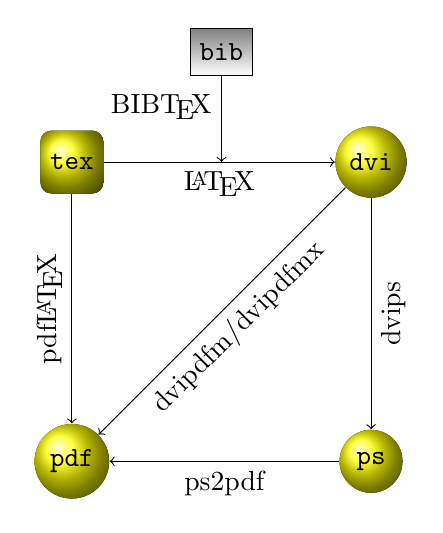
\begin{tikzpicture}
\begin{scope}[shape=circle,minimum size=0.8cm, ball color=yellow]
\tikzstyle{every node}=[fill,shade, rounded corners]
\path (0,3.8) node[shape=rectangle](tex) {\verb|tex|}
      (3.8,3.8) node(dvi) {\verb|dvi|}
      (3.8,0) node(ps)  {\verb|ps|}
      (0,0) node(pdf) {\verb|pdf|};
\end{scope}
\pause
\draw[->] (tex) --node[below]{\LaTeX} (dvi);
\pause
\draw[->] (1.9,5.2) node[draw, minimum size=0.6cm, shape=rectangle,shade](bib){\verb|bib|} -- node[left]{BIB\TeX}(1.9,3.8);
\pause
\draw[->] (dvi) --node[below,rotate=90]{dvips} (ps);
\pause
\draw[->] (ps) --node[below]{ps2pdf} (pdf);
\pause
\draw[->] (tex) --node[rotate=90,above]{pdf\LaTeX} (pdf);
\pause
\draw[->] (dvi) --node[below, sloped]{dvipdfm/dvipdfmx} (pdf);      
    \end{tikzpicture}
\end{minipage}
\begin{minipage}{0.35\linewidth}
\onslide{8-}{\UseVerbatim{mypause}}
\end{minipage}
\end{slide}

\begin{slide}[method=file]{\LaTeX{} 模板使用方法}
\LaTeX{} 定义了四种标准模板:\\
\twocolumn[topsep=0.5cm]{\begin{itemize}
  \item {\color{Bittersweet}article}
  \item \blue{book}
  \end{itemize}}{
\begin{itemize}
  \item report
\item letter
  \end{itemize}}\pause
\begin{MyVerbatim}
\documentclass[12pt]{book}  % 声明模板类型以及相关参数

\author{苏东坡}             % 指定作者
\title{念奴娇 赤壁怀古}     % 指定文章题目

\begin{document}            % 指示正文开始
\maketitle                  % 创建封面

\chapter*{前言}             % 具体章节
\chapter{介绍}
\chapter{详细内容}
\chapter{算法推导}
\chapter{结论}
\end{document}              % 文档结束
\end{MyVerbatim}
\end{slide}

\begin{slide}[toc={命令格式}, method=file]{\TeX{} 和~\LaTeX{} 命令格式}
\mysb{Macro 分类}
\begin{description}
\item[简单命令]
  \begin{itemize}
  \item \verb|\命令|\\\pause
    \verb|{\hei 中国人民解放军}|\pause ~$\Rightarrow$ {\hei 中国人民解放军}\pause 
  \item \verb|\命令{参数}|\\\pause
\verb|\textbf{Bold}| \pause $\Rightarrow$ \textbf{Bold}\pause 
  \item \verb|\命令[参数]|\\\pause 
\verb|\ziju[10pt]|\pause ~$\Rightarrow$ {\ziju[10pt] 增大字距}\pause 
  \end{itemize}
\item[环境] 特殊的命令\\[5pt]\pause 

  \begin{minipage}{0.45\linewidth}
\begin{Verbatim}
\begin{equation*}
  a^2-b^2=(a+b)(a-b)  
\end{equation*}
\end{Verbatim}
  \end{minipage}\pause \hspace{1cm} $ a^2-b^2=(a+b)(a-b)$
\end{description}
\end{slide}

\begin{slide}[method=file]{\LaTeX{} 常用命令}
\mysb{命令}

\centering
% \rowcolors[\hline]{3}{green!25}{yellow!50} \arrayrulecolor{red!75!gray}
\footnotesize
  \begin{tabular}{llll}
    \cmd{chapter} & \cmd{section} & \cmd{subsection} & \cmd{subsubsection} \\
    章 & 节 & 次小节 & 次次小节 \\\hline\pause
    \cmd{textbf} & \cmd{textit} & \cmd{emph} & \cmd{texttt} \\
   粗体 & 斜体 &  强调 & 打字机字体 \\\hline\pause
  \cmd{raggedright} & \cmd{raggedleft} & \cmd{centering} & \cmd{indent}\\
  左对齐 & 右对齐 & 居中对齐 & 段首缩进 \\\hline\pause
  \cmd{footnote} & \cmd{item} & \cmd{caption} & \cmd{includegraphics} \\
   脚注 & 列表条目 & 标题 & 插入图片 \\\hline\pause
  \cmd{label} & \cmd{cite} & \cmd{ref} \\
  标号 & 引用参考文献 & 引用图表公式等\\\hline \pause 
  \end{tabular}
\normalsize
\bigskip

\raggedright\mysb{环境}\pause

\centering
\footnotesize
\begin{tabular}{lll}
  \env{table} & \env{figure} & \env{equation}\\
  表格 & 图片 & 公式 \\\hline
  \env{itemize} & \env{enumerate} & \env{description}\\
  无编号列表 & 编号列表 & 描述 \\\hline
\end{tabular}
\end{slide}

\begin{slide}[method=file]{\LaTeX{} 命令举例}
\cmdxmp{chapter}{前言}{\hei 第~1 章\hspace{1em} 前言}  \pause
\cmdxmp{chapter[精简标题]}{这个题目实在太长了放到目录里面不太好看}{\hei 第~1 章
  \hspace{1em} 这个题目实在太长了放到目录里面不太好看}  \pause

\cmdxmp{section}{背景介绍}{\hei 1.1 \hspace{1em} 背景介绍}  \pause
\cmdxmp{section[精简标题]}{这个题目实在太长了放到目录里面不太好看}{\hei 1.1
  \hspace{1em} 这个题目实在太长了放到目录里面不太好看}  \pause

\twocolumn[topsep=1em]{
\cmdxmp{textbf}{To Bold}{\textbf{To Bold}}\pause
\cmdxmp{textit}{To Italic}{\textit{To Italic}}\pause}{
\cmdxmp{texttt}{To Typeset}{\texttt{To Typeset}}\pause
\cmdxmp{footnote}{脚注说明}{关于质能方程\footnote{$E=mc^{2}$}}}
\end{slide}


\begin{slide}[method=file]{\LaTeX{} 环境命令举例}
  \begin{minipage}{0.4\linewidth}
\begin{MyVerbatim}
\begin{itemize}
  \item 一条
  \item 次条
  \item 再条
\end{itemize}
\end{MyVerbatim}
  \end{minipage}\hspace{1.5cm}
  \begin{minipage}{0.4\linewidth}
\begin{itemize}
  \item 一条
  \item 次条
  \item 再条
\end{itemize}    
  \end{minipage}\pause
\medskip

  \begin{minipage}{0.4\linewidth}
\begin{MyVerbatim}
\begin{enumerate}
  \item 一条
  \item 次条
  \item 再条
\end{enumerate}
\end{MyVerbatim}
  \end{minipage}\hspace{1.5cm}
  \begin{minipage}{0.4\linewidth}
\begin{enumerate}
  \item 一条
  \item 次条
  \item 再条
\end{enumerate}    
  \end{minipage}\pause
\medskip

  \begin{minipage}{0.4\linewidth}
\begin{MyVerbatim}
\begin{description}
  \item[No. 1] 这是一条
  \item[No. 2] 这是次条
  \item[No. 3] 这是再条
\end{description}
\end{MyVerbatim}
  \end{minipage}\hspace{1.5cm}
  \begin{minipage}{0.4\linewidth}
\begin{itemize}
  \item[No. 1] 这是一条
  \item[No. 2] 这是次条
  \item[No. 3] 这是再条
\end{itemize}    
  \end{minipage}
\end{slide}


\begin{slide}[method=file]{自动引用举例~(1)}
  \begin{itemize}
  \item 给对象命名:图片、表格、公式等\\
  \verb|\label{name}|\pause
\item 引用对象\\
  \verb|\ref{name}|\pause
  \end{itemize}
\bigskip

  \begin{minipage}{0.5\linewidth}
\begin{MyVerbatim}
\begin{figure}
  \centering
  \includegraphics{thu-fig-logo.pdf}
  \caption{清华校徽。}
  \label{fig:thulogo}
\end{figure}
清华校徽请参见图~\ref{fig:thulogo}
\end{MyVerbatim}
  \end{minipage}\hfill\pause
  \begin{minipage}{0.4\linewidth}\centering
 \includegraphics[scale=0.1]{thu-fig-logo.pdf}\\
 {\small 图~1. 清华校徽。}\\[1em]
清华校徽请参见图~1。    
  \end{minipage}
\end{slide}

\begin{slide}[method=file]{自动引用举例~(2)}
\begin{minipage}{0.55\linewidth}
  \begin{MyVerbatim}
\begin{table}
   \centering
   \begin{tabular}{ll}\hline
     编号 & 含义 \\\hline
     1 & 第一\\
     2  & 第二\\\hline
   \end{tabular}
   \caption{编号与含义。}
   \label{tab:number}
\end{table}
编号与含义请参见表~\ref{tab:number}。
\end{MyVerbatim}
\end{minipage}\pause
\begin{minipage}{0.4\linewidth}
\centering\small
 \begin{tabular}{ll}\hline
编号 & 含义 \\\hline
1 & 第一\\
2  & 第二\\\hline
\end{tabular}\\[5pt]
{\small 表~1. 编号与含义}\\[1em]
\normalsize 编号与含义请参见表~1。
\end{minipage}\pause

  \begin{MyVerbatim}
\begin{equation}
  \label{eq:sum}
  \sum\limits_{1}^{n}{i}=\frac{n(n+1)}{2}
\end{equation}
公式~\ref{eq:sum} 为等差数列求和。
\end{MyVerbatim}

\pause
\begin{equation}\label{eq:exam}
\sum\limits_{1}^{n}{i}=\frac{n(n+1)}{2}
\end{equation}
公式~\eqref{eq:exam} 为等差数列求和。
\end{slide}

\section{\thuthesis{} 简要说明}

\subsection{\thuthesis{} 的下载与安装}
\begin{slide}{准备工作~(1)}
\mysb{安装~\TeX{} 系统}
  \begin{description}
  \item[Windows] 推荐~C\TeX{}
    \begin{itemize}
    \item 下载~C\TeX:\href{http://www.ctex.org}{www.ctex.org}
    \item 安装:CTeX-full.exe,CTeX-Fonts.exe
    \end{itemize}
  \item[其它] Linux,FreeBSD
    \begin{itemize}
    \item TeXLive
    \end{itemize}
  \end{description}
\end{slide}

\begin{slide}{准备工作~(2)}
\mysb{安装~\thuthesis}
 \begin{description}
 \item[下载] 
   \begin{itemize}
   \item \href{http://thuthesis.sf.net}{http://thuthesis.sourceforge.net}
   \item \href{http://gforge.oss.org.cn/projects/thuthesis/}{http://gforge.oss.org.cn/projects/thuthesis/}
   \end{itemize}
 \item[安装]
   \begin{itemize}
   \item 解压缩参看安装文档~(\Large {\bf\color{red}Readme} 和~{\bf\color{red}thuthesis.pdf})
   \item 养成看文档的好习惯
   \end{itemize}
 \end{description}  
\end{slide}

\begin{slide}[method=direct]{概貌}
\begin{minipage}[t]{0.45\linewidth} 
  \begin{MyVerbatim}[fontsize=\tiny]
\documentclass[bachelor,dvips]{thuthesis}
% \documentclass[bachelor|master|doctor,
%                dvips|dvipdfm,
%                secret,
%                submit,
%                arialtoc,
%                arialtitle]{thuthesis}
% 所有其它可能用到的包都统一放到这里了,
% 可以根据自己的实际添加或者删除。
\usepackage{thutils}

\begin{document}
%%% 封面部分
\frontmatter
\input{data/cover}
\makecover

% 目录
\tableofcontents

% 符号对照表
\input{data/denotation}
\end{MyVerbatim}
\end{minipage}\hfill
\begin{minipage}[t]{0.45\linewidth} 
\begin{MyVerbatim}[fontsize=\tiny]
%%% 正文部分
\mainmatter
\include{data/chap01}
\include{data/chap02}

%%% 其它部分
\backmatter
% 插图索引
\listoffigures
% 表格索引
\listoftables
% 公式索引
\listofequations

% 参考文献
\bibliographystyle{thubib}
\bibliography{ref/refs}

% 致谢
\include{data/ack}

% 附录
\begin{appendix}
\input{data/appendix01}
\end{appendix}

% 个人简历
\include{data/resume}
\end{document}
  \end{MyVerbatim}
\end{minipage}
\end{slide}

\subsection{\thuthesis{} 命令详解}
\begin{slide}[method=direct]{论文选项~(1)}
\mysb{选项}
\begin{description}
\item[bachelor] 我要写本科论文
  \begin{Verbatim}
\documentclass[bachelor]{thuthesis}
  \end{Verbatim}
\item[master] 我要写硕士论文
  \begin{Verbatim}
\documentclass[master]{thuthesis}
  \end{Verbatim}
\item[doctor] 我要写博士论文
  \begin{Verbatim}
\documentclass[doctor]{thuthesis}
  \end{Verbatim}
\item[secret] 论文有保密要求
  \begin{Verbatim}
\documentclass[doctor, secret]{thuthesis}
\secretlevel{机密}
\secretyear{2010}
  \end{Verbatim}
\item[openany, openright] 章节首页是否右开。
\item[dvips, dvipdfm] 使用~dvips/dvipdfm 生成文档。
%\item[submit] 本科论文最终提交
%  \begin{Verbatim}
%\documentclass[bachelor, submit]{thuthesis}
%  \end{Verbatim}
\end{description}
\end{slide}

\begin{slide}{封面样例~(1)}
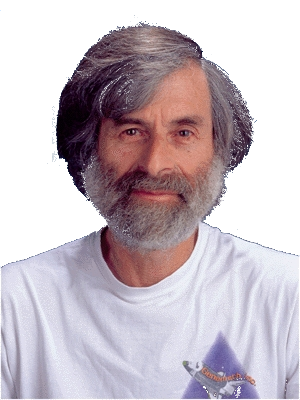
\includegraphics[width=4.5cm]{lamport.png}\hfill%bachelor.eps
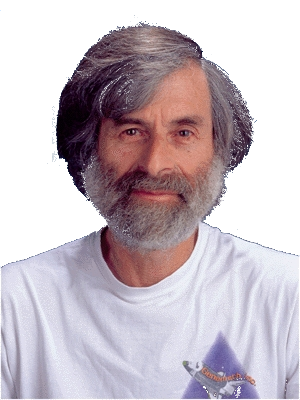
\includegraphics[width=4.5cm]{lamport.png}%master.eps
\end{slide}

\begin{slide}{封面样例~(2)}
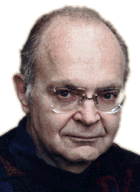
\includegraphics[width=4.5cm]{knuth.png}\hfill%doctor.eps
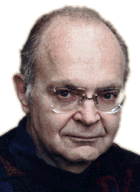
\includegraphics[width=4.5cm]{knuth.png}%doctore.eps
\end{slide}

\begin{slide}[method=direct]{字体切换}
   \begin{tabular}{llllll}
  {\song 宋体} & {\fs 仿宋} & {\hei 黑体} & {\kai 楷体} & {\li 隶书} & {\you 幼圆} \\\hline
  \cmd{song} &\cmd{fs}&\cmd{hei}&\cmd{kai}&\cmd{li}&\cmd{you}\\
  \cmd{songti}&\cmd{fangsong}&\cmd{heiti}&\cmd{kaishu}&\cmd{lishu}&\cmd{youyuan}\\\hline
 \end{tabular}
\bigskip

\mysb{示例}\\[5pt]
\begin{minipage}{0.43\linewidth} 
\begin{MyVerbatim}[baselinestretch=1.4]
{\song 乾:元,亨,利贞} \\
{\fs 初九,潜龙勿用}\\
{\hei 九二,见龙在田,利见大人}\\
{\kai 九三,君子终日乾乾,夕惕若,
           厉,无咎}\\
{\li 九四,或跃在渊,无咎}\\
{\hei 九五,飞龙在天,利见大人}\\
{\song 上九,亢龙有悔}\\
{\you 用九,见群龙无首,吉}
\end{MyVerbatim}
\end{minipage}
\begin{minipage}{0.55\linewidth}  
{\song 乾:元,亨,利贞} \\
{\fs 初九,潜龙勿用}\\
{\hei 九二,见龙在田,利见大人}\\
{\kai 九三,君子终日乾乾,夕惕若,厉,无咎}\\
{\li 九四,或跃在渊,无咎}\\
{\hei 九五,飞龙在天,利见大人}\\
{\song 上九,亢龙有悔}\\
{\you 用九,见群龙无首,吉}
\end{minipage}
\end{slide}

\begin{slide}[method=direct]{字号切换}
 \begin{tabular}{lllll}\hline
 \cmd{chuhao}&\cmd{xiaochu}&\cmd{yihao}&\cmd{xiaoyi} &\\
  \cmd{erhao}&\cmd{xiaoer}&\cmd{sanhao}&\cmd{xiaosan}&\\
 \cmd{sihao}& \cmd{banxiaosi}&\cmd{xiaosi}&\cmd{dawu}&\cmd{wuhao}\\
 \cmd{xiaowu}&\cmd{liuhao}&\cmd{xiaoliu}&\cmd{qihao}& \cmd{bahao}\\\hline
 \end{tabular}
\bigskip 

\mysb{使用方法}
\begin{itemize}
\item \verb|\command[num]|
\item \cmd{command} 为字号命令,\verb|num| 为行距。
\item \verb|\xiaosi[1.5]| 表示选择小四字体,行距~1.5 倍。
\end{itemize}

\begin{MyVerbatim}
  {\erhao 二号 \sanhao 三号 \sihao 四号  \qihao 七号}
\end{MyVerbatim}
  {\erhao 二号 \sanhao 三号 \sihao 四号  \qihao 七号}
\end{slide}

\begin{slide}[method=direct]{封面}
\footnotesize
  \begin{tabular}{lll}
    命令作用 & 中文命令 & 英文命令 \\\hline\hline
  论文标题 & \cmd{ctitle} &\cmd{etitle}\\
  作者姓名&  \cmd{cauthor} &\cmd{eauthor}\\
  申请学位名称 & \cmd{cdegree}&\cmd{edegree}\\
  院系名称 & \cmd{cdepartment} & \cmd{edepartment}\\
  专业名称 & \cmd{cmajor} & \cmd{emajor}\\
  导师 & \cmd{csupervisor} & \cmd{esupervisor}\\
  副导师 & \cmd{cassosupervisor} & \cmd{eassosupervisor}\\
  联合导师 & \cmd{ccosupervisor} & \cmd{ecosupervisor}\\
  日期 & \cmd{cdate} & \cmd{edate}\\
  摘要 & \cmd{cabstract} & \cmd{eabstract}\\
  关键词 & \cmd{ckeywords} & \cmd{ekeywords}\\\hline
  \end{tabular}
\normalsize
\bigskip

\mysb{示例}
\begin{MyVerbatim}
\ctitle{\thuthesis{} 从入门到精通} 
\etitle{Mastering \thuthesis}
\cauthor{薛瑞尼} 
\eauthor{Xue Ruini}
\end{MyVerbatim}
\vspace*{-1.7em}
\begin{itemize}
\item {\color{red}请参看示例文档!}
\end{itemize}
\end{slide}

%\begin{slide}[method=file]{杂项}
%  \begin{description}
%  \item[符号对照表] \\[3pt]
%    \begin{minipage}{0.4\linewidth}
%\begin{MyVerbatim}
%\begin{denotation}
%\item[E] 能量
%\item[m] 质量
%\item[c] 光速
%\end{denotation} 
%    \end{MyVerbatim}
%\end{minipage}\hspace{1cm}\pause
%\begin{minipage}{0.4\linewidth}
%{\hei\wuhao 主要符号对照表}
%\begin{tabular}{ll}
%E &  能量 \\
%m & 质量 \\
%c & 光速 \\  
%\end{tabular}
%\end{minipage}
%\end{description}\pause
%
%\begin{minipage}[t]{0.45\linewidth}
%\begin{description}
%\item[致谢与声明] \\
%  \begin{MyVerbatim}
%\begin{ack}    
%感谢天,感谢地,感谢风调雨顺!
%\end{ack}
%  \end{MyVerbatim}
%\end{description}
%\end{minipage}\pause
%\begin{minipage}[t]{0.45\linewidth}
%\begin{description}
%\item[附录] \\
%  \begin{MyVerbatim}
%\begin{appendix}
%\input{data/appendix01}
%\end{appendix}    
%  \end{MyVerbatim}
%\end{description}
%\end{minipage}\pause
%
%\begin{minipage}[t]{0.6\linewidth}
%\begin{description}
%\item[简历] \\
%  \begin{MyVerbatim}
%\begin{resume}
%\resumeitem{个人简历}
%  xxxx
%\resumeitem{目前已正式发表的论文}
%  yyyy
%\end{resume}
%  \end{MyVerbatim}
%  \end{description}
%\end{minipage}
%\end{slide}

\begin{slide}[method=file]{数学相关}
  \begin{itemize}
  \item \TeX{} 的强项在于处理数学公式
  \item \thuthesis{} 定义了常用的数学环境:\\[10pt]

    \begin{tabular}{lllll}\hline
axiom & theorem & definition & proposition & lemma \\
公理 & 定理 & 定义 & 命题 & 引理 \\\hline
proof & corollary & example & exercise &\\
证明 & 推论 & 例子& 练习 &\\\hline
    \end{tabular}
  \end{itemize}\pause
\bigskip

\mysb{示例}

\begin{MyVerbatim}
\begin{definition}
道千乘之国,敬事而信,节用而爱人,使民以时。
\end{definition}
\end{MyVerbatim}

{\hei 定义~1.1~~~~} {\song 道千乘之国,敬事而信,节用而爱人,使民以时。}
\end{slide}

\begin{slide}[method=file]{参考文献}
\mysb{BIB\TeX}
  \begin{itemize}
  \item 参考文献管理自动化
  \item bib 文件
  \item bst 参考文献样式文件:thubib.bst
  \item 学校要求两种引用方式:\pause
    \begin{itemize}
    \item 上标模式:如“在许多文献$^{[12,13]}$中……”
      \begin{Verbatim}
\cite{key12, key13}        
      \end{Verbatim}
\pause
    \item 正文模式:如“文献~[14] 证明了……”
      \begin{Verbatim}
\onlinecite{key14}        
      \end{Verbatim}
    \end{itemize}
  \end{itemize}
\end{slide}

\begin{slide}{关于作图}
  \begin{description}
  \item[矢量图] eps, ps, pdf
    \begin{itemize}
    \item \MP,pstricks,pgf $\ldots$
    \item Xfig,Dia,Visio,Inkscape $\ldots$
    \end{itemize}
  \item[标量图] png,jpg,tiff $\ldots$
  \item[转化]
\twocolumn{
    \begin{itemize}
    \item 虚拟打印机
    \item ImageMagick
    \end{itemize}}{
    \begin{itemize}
    \item GSViewer
    \item 其它:epstopdf,pdfcrop
    \end{itemize}}
  \end{description}

\medskip
\includegraphics[scale=0.25]{thu-lib-logo.pdf}\hspace{2cm}\includegraphics[scale=0.7]{thu-lib-logo.pdf}
\end{slide}

\section[toc=深入~\thuthesis]{一步一步掌握~\thuthesis}

\begin{slide}{目录}
  \begin{itemize}
  \item 详细介绍使用~\thuthesis{}
    \begin{itemize}
    \item 模板结构
    \item 封面
    \item 主要符号表
    \item 章节
    \item 致谢
    \item 附录
    \item 索引
    \item 简历
    \item 书脊
    \end{itemize}
  \end{itemize}
\end{slide}

\begin{slide}[method=file]{\thuthesis{} 的结构}
  \begin{minipage}[t]{0.6\linewidth}    
  \begin{itemize}
  \item \thuthesis{} 包括以下文件
  \end{itemize}
  \begin{tabular}{ll}
      {\hei 文件} & {\hei 说明}\\\hline
thuthesis.ins & 安装辅助文件\\
thuthesis.dtx & 模板源文件 \\
thuthesis.cls & 模板核心文件 \\
thuthesis.cfg & 模板配置文件 \\
thubib.bst & 参考文献样式文件 \\
Readme & 简单说明文档 \\
thuthesis.pdf & 用户手册
    \end{tabular}
  \end{minipage}\pause
  \begin{minipage}[t]{0.38\linewidth}  
    \begin{itemize}
    \item 推荐结构
    \end{itemize}
    \begin{YourVerbatim}
thesis/ 
  |- thuthesis.cls
  |- thuthesis.cfg
  |- thubib.bst   
  |- thutils.sty  
  |- main.tex
  |- data/
       |- cover.tex
       |- denotation.tex
       |- chapter01.tex
       |- ack.tex
       |- resume.tex
       |- appendix.tex  
  |- ref/
      |- ref.bib
  |- figures/
      |- xrn.eps
    \end{YourVerbatim}
  \end{minipage}
\end{slide}

\begin{slide}[method=direct]{概貌}
\begin{minipage}[t]{0.45\linewidth} 
\begin{MyVerbatim}[fontsize=\tiny]
\documentclass[bachelor,dvips]{thuthesis}
% \documentclass[bachelor|master|doctor,
%                dvips|dvipdfm,
%                secret,
%                submit,
%                arialtoc,
%                arialtitle]{thuthesis}
% 所有其它可能用到的包都统一放到这里了,
% 可以根据自己的实际添加或者删除。
\usepackage{thutils}

\begin{document}
%%% 封面部分
\frontmatter
\input{data/cover}
\makecover

% 目录
\tableofcontents

% 符号对照表
\input{data/denotation}
\end{MyVerbatim}
\end{minipage}\hfill
\begin{minipage}[t]{0.45\linewidth} 
  \begin{MyVerbatim}[fontsize=\tiny]
%%% 正文部分
\mainmatter
\include{data/chap01}
\include{data/chap02}

%%% 其它部分
\backmatter
% 插图索引
\listoffigures
% 表格索引
\listoftables
% 公式索引
\listofequations

% 参考文献
\bibliographystyle{thubib}
\bibliography{ref/refs}

% 致谢
\include{data/ack}

% 附录
\begin{appendix}
\input{data/appendix01}
\end{appendix}

% 个人简历
\include{data/resume}
\end{document}
  \end{MyVerbatim}
\end{minipage}
\end{slide}

\subsection{封面}

\begin{slide}[method=file]{封面示例~(1)}
\def\mytwocolumn<#1>#2{%
\twocolumn[lcolwidth=0.65\linewidth,rcolwidth=0.32\linewidth]%
  {\mypauseverb<#1>{\UseVerbatim{mypause}}}
  {#2}}
\pause
\begin{SaveVerbatim}[commandchars=!\[\]]{mypause}
% 定义密级
\secretlevel{[机密]} \secretyear{[2020]}
\end{SaveVerbatim}
\mytwocolumn<2->{\myitem<2->{密级}}
\begin{SaveVerbatim}[commandchars=!\[\]]{mypause}
% 定义题目
\ctitle{[!red[清华大学学位论文~\LaTeX\ 模板使用示例文档]]}
\etitle{[!red[An Introduction to \LaTeX{}]]
        [!red[Thesis Template of Tsinghua University]]}
  \end{SaveVerbatim}
\mytwocolumn<3->{\myitem<3->{论文题目}}
  \begin{SaveVerbatim}[commandchars=!\[\]]{mypause}
% 作者和导师信息
\cauthor{[!red[薛瑞尼]]} 
\eauthor{[!red[Xue Ruini]]} 
\csupervisor{[!red[郑纬民教授]]}
\esupervisor{[!red[Professor Zheng Weimin]]} 
\cassosupervisor{[!red[[陈文光副教授]]}
\eassosupervisor{[!red[Chen Wenguang]]} 
\ccosupervisor{[!red[[某某某教授]]}
\ecosupervisor{[!red[I have no]]}
  \end{SaveVerbatim}
\mytwocolumn<4->{\myitem<4->{作者和导师信息}}
  \begin{SaveVerbatim}[commandchars=!()]{mypause}    
% 学位与专业信息
\cdegree{(!red[工学博士])} 
\edegree{(!red(Doctor of Science))} 
\cdepartment(!hei!blue[计算机]){(!red[计算机科学与技术系])} 
\cmajor{(!red[计算机科学与技术])}
\emajor{(!red(Computer Science and Technology))} 
\end{SaveVerbatim}
\mytwocolumn<5->{\myitem<5->{学位与专业}\myitem<6->{日期会自动设置为当前日期\\ (\cmd{cdate}~\cmd{edate})}}
\end{slide}

\begin{slide}[method=file]{封面示例~(2)}
\pause
 \begin{SaveVerbatim}[commandchars=!\[\]]{mypause}
% 中英文摘要
\cabstract{本文介绍清华大学论文~\LaTeX + CJK 模板的使用方法。本模板基本符合学校
  的博士、硕士论文格式要求。具体使用方法请参看本文源文件。}
\eabstract{This article presents the \LaTeX + CJK template for Master Thesis of
  Tsinghua University, and briefly introduces the usage.}
\end{SaveVerbatim}
\mypauseverb<2->{\UseVerbatim{mypause}}
 \begin{SaveVerbatim}[commandchars=!\[\]]{mypause}
% 中英文关键词
\ckeywords{\TeX,\LaTeX,CJK,模板,排版,论文}
\ekeywords{\TeX,\LaTeX,CJK,template,typesetting,thesis}
\end{SaveVerbatim}
\mypauseverb<3->{\UseVerbatim{mypause}}
\medskip

\myitem<2->{中英文摘要}
\myitem<3->{中英文关键词}
\myitem<4->{\cmd{makecover} 自动生成封面}
\end{slide}


%\begin{slide}[method=direct]{封面示例~(3)}
%\mysb{综合论文训练任务书新增内容}\\[10pt]
%
%\twocolumn{%
%    \begin{itemize}
%    \item 学生号
%    \item 班级号
%    \item 同组成员
%    \end{itemize}
%}{%
%  \begin{itemize}
%  \item 主要进度
%  \item 主要要求(指标)
%  \item 主要参考文件
%  \end{itemize}
%}
%\begin{MyVerbatim}
%\studentid{2005310432}
%\classid{计研~2}
%\groupmemebers{edyfox}
%
%\contentsandprogress{这是主要进度}
%\mainrequirements{这是主要要求(指标)}
%\mainreferences{这是主要参考文献}
%\end{MyVerbatim}
%\begin{itemize}
%\item 提交论文时签字图片
%\end{itemize}
%\begin{MyVerbatim}
%\bachelorcommentsfig{hello.eps}   % 教师评语部分
%\bachelorauthfig[scale=2]{hello.eps} % 论文授权说明部分
%\bacheloroverviewfig[width=0.5\textwidth]{hello.eps} % 综合论文训练部分
%\bachelordeclarefig[height=4cm]{hello.eps} % 声明部分
%\end{MyVerbatim}
%\end{slide}


\subsection{主要符号表}
\begin{slide}[method=file]{主要符号表}
  \begin{MyVerbatim}
\begin{denotation}
\item[E]   能量
\item[m]   质量
\item[c]   光速
\end{denotation}
  \end{MyVerbatim}
  \begin{itemize}
  \item 每个条目由两部分组成:
  \item (key, value)
  \end{itemize}
\end{slide}

\subsection{正文}
\begin{slide}[method=file]{章节细节}
\pause
\begin{SaveVerbatim}{mypause}
\chapter{雷锋塔的倒掉}  
\label{cha:lft}
\end{SaveVerbatim}
\twocolumn[lcolwidth=0.35\linewidth,rcolwidth=0.6\linewidth]%
  {\mypauseverb<2->{\UseVerbatim{mypause}}}
  {\myitem<2->{章:{\hei 第三章\hspace{1em}雷锋塔的倒掉}}}
\begin{SaveVerbatim}{mypause}  
\section{雷锋塔的历史}
\label{sec:lfthist}
\end{SaveVerbatim}
\twocolumn[lcolwidth=0.35\linewidth,rcolwidth=0.6\linewidth]%
  {\mypauseverb<3->{\UseVerbatim{mypause}}}
  {\myitem<3->{节:{\hei 3.1\hspace{1em}雷锋塔的历史}}}
\begin{SaveVerbatim}{mypause}
\subsection{谁修建的雷锋塔}
\label{sec:whobuildlft}
\end{SaveVerbatim}
\twocolumn[lcolwidth=0.35\linewidth,rcolwidth=0.6\linewidth]%
  {\mypauseverb<4->{\UseVerbatim{mypause}}}
  {\myitem<4->{小节:{\hei 3.1.1\hspace{1em}谁修建的雷锋塔}}}
\begin{SaveVerbatim}{mypause}    
\subsubsection{钱王与保叔塔}
\label{sec:sonofkingofmoney}}
\end{SaveVerbatim}
\twocolumn[lcolwidth=0.35\linewidth,rcolwidth=0.6\linewidth]%
  {\mypauseverb<5->{\UseVerbatim{mypause}}}
  {\myitem<5->{次小节:{\hei 3.1.1.1\hspace{1em}钱王与保叔塔}}}
\begin{SaveVerbatim}{mypause}  
\chapter{雷锋塔倒掉之后的故事}  
\label{cha:afterlft}
\section{白娘子哪里去了?}
\label{sec:whereismzbai}
\section{法海呢?}
\label{sec:whereisfahai}
\subsection{螃蟹的故事}
\label{sec:storyofcrab}
\end{SaveVerbatim}
\twocolumn[lcolwidth=0.35\linewidth,rcolwidth=0.6\linewidth]%
  {\mypauseverb<6->{\UseVerbatim{mypause}}}
  {\myitem<6->{同上}}
\end{slide}


\subsection{致谢与声明}
\begin{slide}[method=direct]{致谢}
  \begin{itemize}
  \item 简单致谢的环境
  \item 声明部分会自动生成
  \end{itemize}
  \begin{MyVerbatim}
\begin{ack}
本科的致谢和声明分页,硕士博士不分。

所以本科可以多写一些,研究生少写一些。
\end{ack} 
  \end{MyVerbatim}
\end{slide}

\subsection{附录}
\begin{slide}[method=direct]{附录}
  \begin{MyVerbatim}
\begin{appendix}
\chapter{中心极限定理的证明}    
\section{问题描述}
Anything as you like...
\end{appendix}
  \end{MyVerbatim}
  \begin{itemize}
  \item 用~\verb|appendix| 环境
  \item 与普通章节没有任何区别
  \item 模板自动修改章名为:{\hei 附录~~A}
  \end{itemize}
\end{slide}

\subsection{插图、表格、公式索引}
\begin{slide}[method=direct]{三种索引}
\begin{itemize}
\item 插图索引:\verb|\listoffigures|
\item 表格索引:\verb|\listoftables|
\item 公式索引:\verb|\listofequations|
\end{itemize}

\bigskip
\mysb{公式编号}
\begin{itemize}
\item \LaTeX 默认不提供公式索引
\item \thuthesis 提供了命令~\verb|\equcaption| 将公式编号写入临时文件,并由~\verb|\listofequations| 生成。
\end{itemize}
\begin{MyVerbatim}
\begin{align} 
  \label{eq:emc2}\equcaption
  E=mc^2
\end{align}
\end{MyVerbatim}
\end{slide}

\subsection{个人简历}
\begin{slide}[method=direct]{个人简历}
  \begin{MyVerbatim}[]    
\begin{resume}
\resumeitem{个人简历} 
  1978 年~4 月~30 日出生于花果山水帘洞,1996~年~9~月考入花果山大学中文专业,
  2000~年~6~月本科毕业并获得文学学士学位,同年~9~月免试保送清华大学应用魔法系攻
  读博士至今。

\resumeitem{目前已正式发表的论文}
  \begin{enumerate} 
  \item Harry Potter, Bajie Zhu, Sanzang Tang, Coupling Computation of the BEM
    and FDM in 3D Spirit Extraction, Interplanetarian Conference on Super 
    Sudden Motion, 2001, p.716 - 719(SCI).
  \end{enumerate}

\resumeitem{目前已被录用文章}
  \begin{enumerate}
  \item Wukong Sun, Harry Potter, Sanzang Tang, Fast 6-D Impedance Extraction 
    of Spirit, International Conference on Communication, Circuit and Systems,
    2005, 已录用.
\end{enumerate}
\end{resume}  
\end{MyVerbatim}
\begin{itemize}
\item 简历环境:\verb|resume|
\item 简历子条目:\cmd{resumeitem}
\end{itemize}
\end{slide}


\subsection{书脊}
\begin{slide}[method=file]{书脊}
  \begin{description}
  \item[书脊] 生成书脊
    \begin{MyVerbatim}
\documentclass{thuthesis}
\begin{document}
\ctitle{\thuthesis{} 从入门到精通}
\cauthor{薛瑞尼}
% \shuji 命令需要上面两个变量
\shuji
\end{document}  
    \end{MyVerbatim}
  \end{description}
\end{slide}

\section{总结}
\begin{slide}{常见问题}
  \begin{description}
  \item[编译不通过] 缺少必要宏包
  \item[标点符号出现在行首] 缺少~CJKpunct 宏包或者安装不对
  \item[表格图片乱跑] \LaTeX{} 自身的~float 定位算法
  \item[段落间距变大] \LaTeX{} 排版算法
  \item[参考文献] 推荐使用~BIB\TeX{},或者自己写
  \item[生成~ps 文件特别大] 字体安装有问题
  \end{description}
\end{slide}

\begin{slide}[method=file]{一点建议}
\mysb{先学习}
  \begin{itemize}
  \item 仔细阅读《一份不太简短的~\LaTeXe{} 介绍》~(1--2 天)
  \item 粗略阅读《\LaTeXe{} 插图指南》~(2--3 小时)
  \item 仔细阅读《\thuthesis{} 用户手册》~(20 分钟)
  \item 从~\thuthesis{} 示例文档入手
  \item 选择一个好编辑器
    \begin{itemize}
    \item 初级用户:WinEdt$\ldots$ 
\includegraphics[scale=0.2]{emacs.png}%winedt.eps
    \item 进阶用户:Vim (+ \LaTeX Suite) 
\includegraphics[scale=0.16]{emacs.png}%vim.eps
    \item 高级用户:Emacs (+ AUC\TeX + preview-\LaTeX) 
\includegraphics[scale=0.16]{emacs.png}
    \end{itemize}
  \end{itemize}
\end{slide}

\begin{slide}[method=file]{求助}
\mysb{如果遇到问题}
\begin{itemize}
\item 阅读文档~(RTFM) 
\item {\color{blue} google}
\item 到~\TeX @newsmth 查找或发文
\item 到~\href{http://groups.google.com/group/thuthesis}\thuthesis{} Google Group 发问
\item 给我写信~$\Rightarrow$ {\hei 不推荐}
\end{itemize}\pause
\bigskip

\mysb{需要你的帮助}
\begin{itemize}
\item 错误反馈
\item 改进建议
\item 出力维护
\item 感谢:\textbf{\color{blue} oseen, donated, edyfox, Truel}
\end{itemize}
\end{slide}

\begin{slide}{谢谢!}
\vspace{\stretch{2}}
\centering
  \includegraphics[width=5cm]{thanks.pdf}
\vspace{\stretch{3.5}}
\end{slide}
\end{CJK*}
\end{document}
